%
%
In this section, we give specifics on the matrices representing the various maps needed in the loss function computation. 

\subsubsection{Boundary Matrices}
\label{ssec:BdyMatrices}
%
    \begin{figure}[]
        \centering
        %
        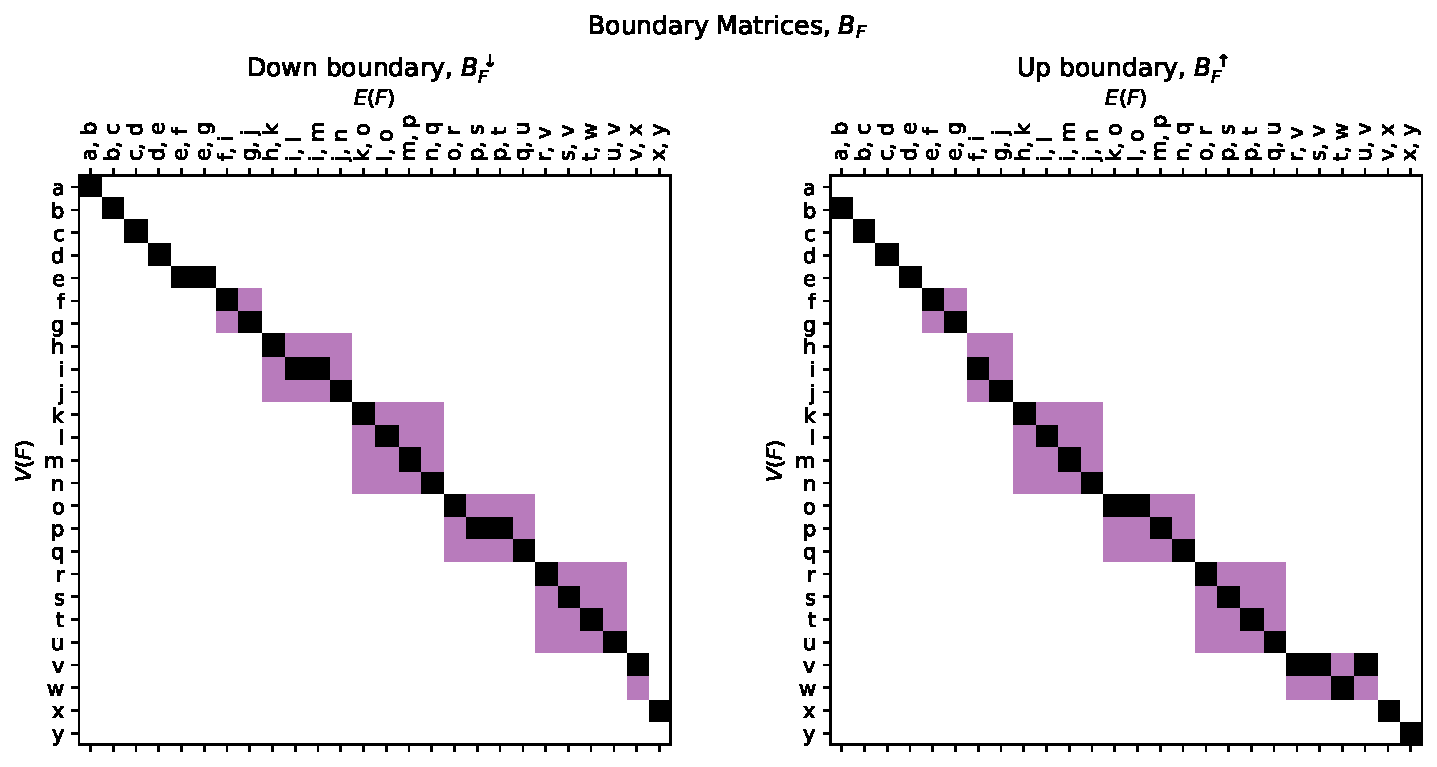
\includegraphics[width = .8\textwidth, align = c]{figures/interleave_example_boundary_matrices.pdf}
        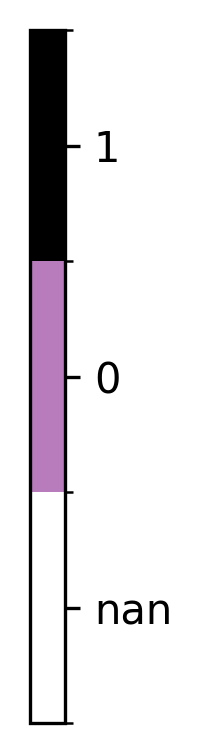
\includegraphics[width = .07\textwidth, align = c]{figures/colorbar-PurBl-binary.png}
        \caption{Example boundary matrices of the graph of $F$ shown in \cref{fig:example_all_graphs}.}
        \label{fig:boundary_matrix}
    \end{figure}
    %
The boundary matrices describe the relationship between the edges and vertices of a graph representation of a given mapper cosheaf. 
For a mapper cosheaf $H \in \{F, F^n,  G, G^n \}$, this is a matrix $B_H \in \{0,1\}^{|E_H| \times |V_H|}$, with a 1 in entry $B_H[e,v]$ iff $v$ is an endpoint of $e$. 
Unlike the other matrices we have used, this matrix has two nonzero entries in each column. However, it can be decomposed into a sum of two block matrices, each with a single nonzero entry per column, as follows. 
Let $B_H^{\uparrow} \in \{0,1\}^{|E_H| \times |V_H|}$ have a 1 in entry $B[e,v]$ iff $v$ is an endpoint of $e$ for $v \in F(\sigma_i)$ and $e \in F(\tau_{i})$; let $B_H^{\downarrow} \in \{0,1\}^{|E_H| \times |V_H|}$ have a 1 in entry $B[e,v]$ iff $v$ is an endpoint of $e$ for $v \in F(\sigma_i)$ and $e \in F(\tau_{i-1})$. 
Then $B_H = B_H^{\uparrow} + B_H^{\downarrow}$; see \cref{fig:boundary_matrix} for an example. 
In this case, we will have eight matrices to work with, which we denote by 
$B_F^{\uparrow}$, $B_F^{\downarrow}$, 
$B_{F^n}^{\uparrow}$,  $B_{F^n}^{\downarrow}$,  
$B_G^{\uparrow}$, $B_G^{\downarrow}$, 
$B_{G^n}^{\uparrow}$, and $B_{G^n}^{\downarrow}$.
We do not compute the boundary matrices for either $F^{2n}$ or ${G}^{2n}$ since, as can be seen in \cref{tab:theList}, these matrices are never used.
Because these are simply matrix encodings of the adjacency information of the relevant graphs, they can be constructed in $O(V_{\max} \cdot E_{\max})$ time, where $V_{\max} = \max\{|V_H| \mid H \in F, F^n,  G, G^n  \}$ and $E_{\max} = \max\{|E_H| \mid H \in F, F^n,  G, G^n  \}$.


    %
    %
    %
    %

    %
    %
    %
    %
    %
    %
    %
    %
    %
    %

  %
\subsubsection{Inclusion Matrices} 
\label{ssec:InclusionMatrices}
%
    \begin{figure}[!htb]
        \centering
        %
        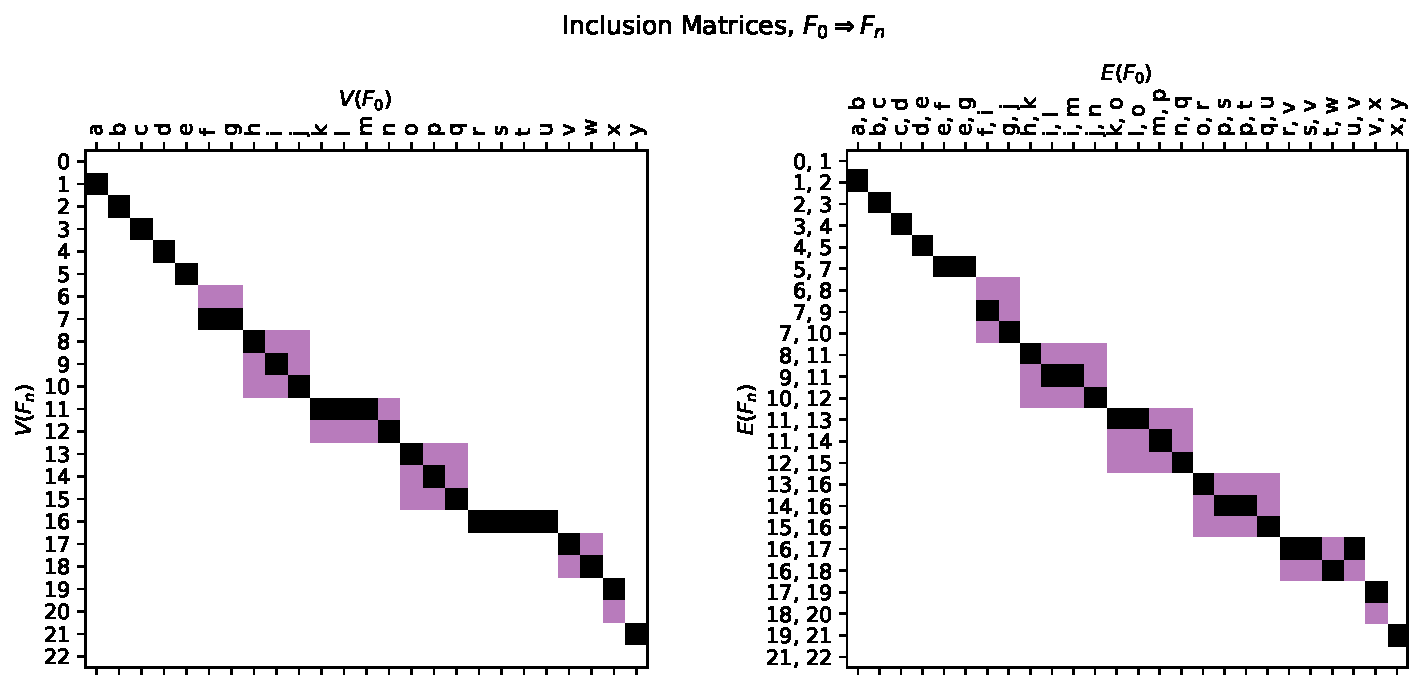
\includegraphics[width = .8\linewidth, align = c]{figures/interleave_example_inclusion_matrices.pdf}
        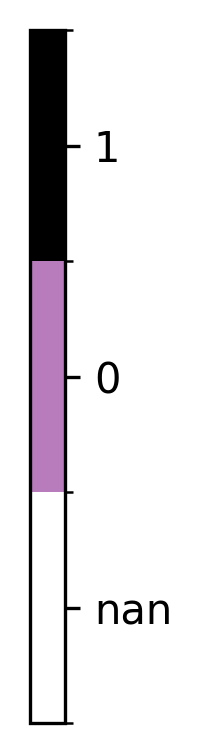
\includegraphics[width = .07\textwidth, align = c]{figures/colorbar-PurBl-binary.png}
        \caption{Inclusion matrices $I_F^V$ (left) and $I_F^E$ (right) representing $F \Rightarrow F_n$ from \cref{fig:example_all_graphs}.}
        \label{fig:inclusion_matrix}
    \end{figure}

The inclusion matrices represent the natural transformations $F \Rightarrow F_n \Rightarrow F_{2n}$ and $G  \Rightarrow G_n  \Rightarrow G_{2n}$.
Focusing on the first of these, $F \Rightarrow F^n$, the component morphisms take a vertex $v \in F(S_{\sigma_i})$ to the vertex $v' \in F^n(S_{\sigma_i})$ representing the connected component containing $v'$. 
The edge maps are determined similarly. 
    Thus the vertex inclusion matrix is written as $I_F^V \in \{0, 1 \}^{|V_{F^n}| \times |V_{F}|}$ with a 1 in entry $I_F[v',v]$ if $v$ is in the connected component represented by $v'$.
    A similar matrix is built for the edges, $I_F^E \in \{0, 1 \}^{|E_{F^n}| \times |E_{F}|}$. 
    The result is that each inclusion natural transformation is given by a pair of matrices, so from this construction we have the matrices $I_F^V$, $I_F^E$, $I_{F^n}^V$, $I_{F^n}^E$, $I_G^V$, $I_G^E$, $I_{G^n}^V$, $I_{G^n}^E$; see \cref{fig:inclusion_matrix} for an example. 
These matrices satisfy the block decomposition and have exactly one nonzero entry in each column. They also have the useful property that the inclusion functor from a graph to its $2n$-smoothing can be computed via matrix multiplication; for example, the induced map on vertices for $F \Rightarrow F_{2n}$ is given by $I_{F^n}^V I_F^V$. Moreover, since they track representatives of objects in the $n$-smoothed connected components, these matrices can be constructed alongside the smoothed graphs with only constant overhead. 

    

    

    
    
    %
    %
    %
    %
    %

    %


%
\subsubsection{Distance Matrices}
%
\label{ssec:DistanceMatrices}
     \begin{figure}[!htb]
       \centering
        %
        %
        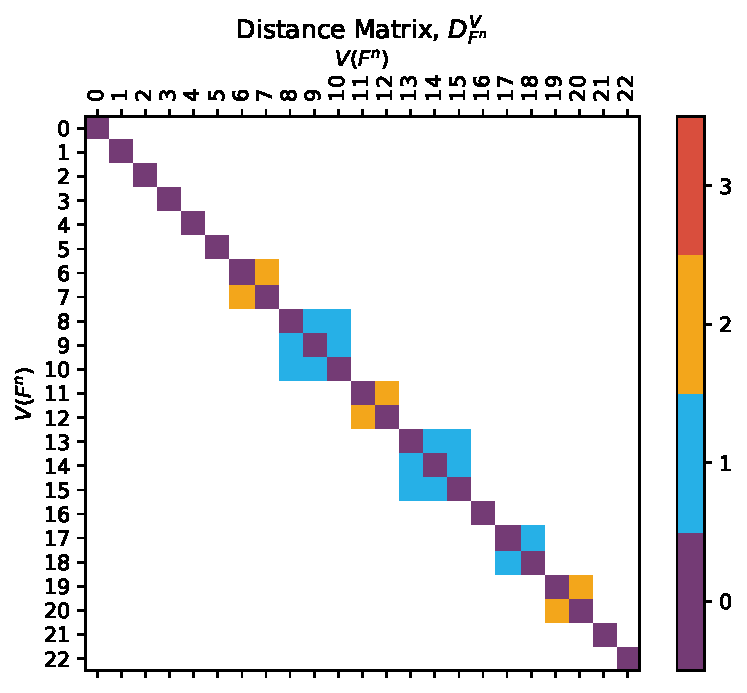
\includegraphics[width = .4\linewidth, align = c]{figures/interleave_example_distance_matrix.pdf}
        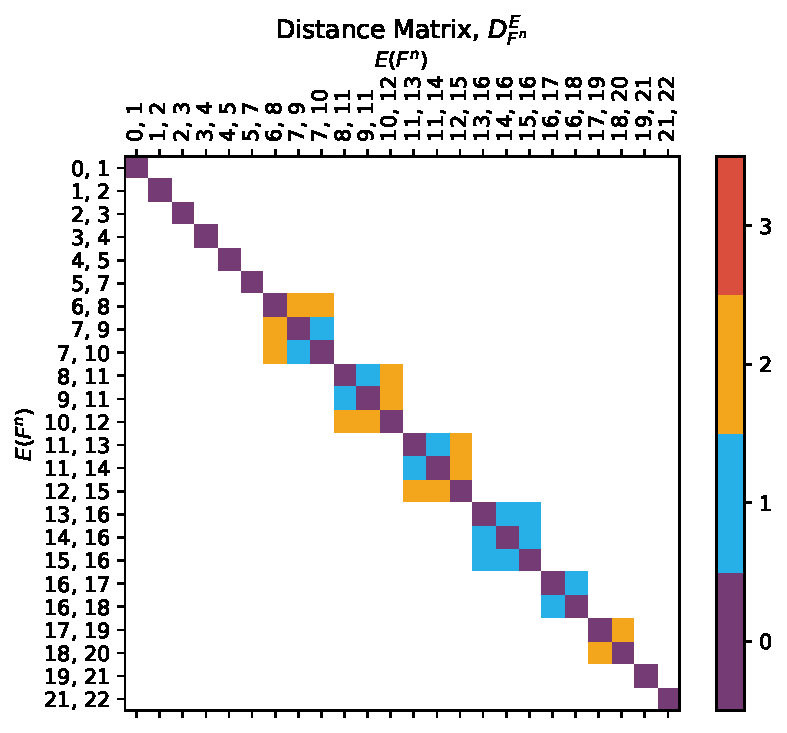
\includegraphics[width = .4\linewidth, align = c]{figures/interleave_example_distance_matrix_edges.pdf}
        \caption{Distance matrix example for $F^n$ from \cref{fig:example_all_graphs}.}
        \label{fig:distance_matrix}
    \end{figure}
The distance matrices encode the distance from \cref{eqn:DistanceDefinition}. 
In particular, for vertices $v,w \in F(S_\rho)$, we seek the minimum $k$ such that they map to the same object in $F(S_\rho^k)$. 
Equivalently, this is the minimum $k$ where $v$ and $w$ are in the same connected component of the subgraph induced by the vertex set $\coprod_{S_{\sigma_i} \subseteq S_\rho^k} F(S_{\sigma_i})$.
For example, in the graph of $F^n$ from \cref{fig:example_all_graphs}, vertices $11$ and $12$, both at level $\sigma_9$, are not in the same connected component until $k=2$ using the path through vertex $7$ below. 
Similarly, edges $(12,15)$ and $(11,14)$ have distance 2 via the path through vertex $7$.


This distance is stored as a pair of matrices $D_F^V \in \{0,1\}^{|V(F)|^2}$ and $D_F^E\in \{0,1\}^{|E(F)|^2}$. 
For the vertices, $D_F^V[u,v] = d_{S_{\sigma_i}}(u,v)$ if $u,v \in F(S_{\sigma_i}) \subset V_F$, and 0 otherwise; $D_F^E$ is defined similarly for the elements of $F(S_{\tau_i})$.
These matrices inherit the block structure determined by the mapper cosheaf heights.
See \cref{fig:distance_matrix} for examples corresponding to $F^n$ from \cref{fig:example_all_graphs}. 
In total, we have 12 distance matrices, two each for the six input matrices. 
However, as noted in \cref{tab:theList}, only the eight for $F^n$, $F^{2n}$, $G^n$, and $G^{2n}$ need to be calculated. 

We now compute these distance matrices from the graph representations.
For each level $i \in [-L,L]$, we construct the block for $\sigma_i$ and $\tau_i$ in $D_F^V$  and $D_F^E$ respectively.
In the vertex case, we build a union-find data structure by adding the edges in order of increasing thickening. 
Recall (and see \cref{fig:PosetNotation} for notation reminder) that the elements of $F(S^k_{\sigma_i})$ correspond to the subgraph induced by the vertices in $\coprod _{j \in [i-n,i+n]} F(S_{\sigma_j})$, which includes the edges in $\coprod_{j \in [i-k, i+k-1]}F(S_{\tau_j})$. 
Therefore, for $k=1$, we add all edges corresponding to $\tau_{i-1}$ and $\tau_i$. Note that the edges for $\tau_{i-2}$ and $\tau_{i+1}$ are irrelevant here, as they do not involve any vertices in $S_{\sigma_j}^1$ and thus cannot affect connectivity. We then check whether any vertices in $F(S_{\sigma_i}^1)$ lie in the same connected component. For each pair $u$ and $v$ that do, we set $D_F^V[u,v] = 1$.
Then for $k=2$, we add the edges for $\tau_{i-2}$ and $\tau_{i+2}$, and repeat the same check for pairs that are not already in the same connected component at $k=1$, setting these distances to 2 if they are now in the same component. 
We continue until all pair distances are determined. 

A similar sweep for each level is used to construct $D_F^E$, with the difference being that the edges added at step $k$ are those from $F(\tau_{i-k+1}, \tau_{i+k-1})$. 
We have $V_{\max}$ entries in our union-find data structure, so amortized time per operation is $O(\alpha(V_{\max}))$, with a total of $E_{\max}$ operations.
Thus, since the union-find structure is built at each level, the pair of matrices for a given graph takes time $O(L\cdot E_{\max} \cdot \alpha(V_{\max}))$, where $\alpha(\cdot)$ is the inverse Ackermann function. 
